\chapter{Поляризационные эффекты и их применение для определения энергии пучка}
\label{sec:respnant_dep}
\section{Радиационная поляризация}
Эффект самопроизвольной поляризации заряженных частиц в ускорителях был описан Соколовым и Терновым еще в 1963г \cite{SokolovTernov63}. Качественно данный эффект можно описать следующим обоазом: в магнитном поле $\vec{H}$ потенциальная энергия частицы с магнитным моментом  $\vec{\mu}$ выражается как: 
\begin{equation}
U = - (\vec{\mu}, \vec{H}).
\end{equation} 
В случае поляризации пучка в ускорителе, $\vec{H}$ есть ведущее поле. Минимум потенциальной энергии дает значение угла между магнитным моментом и ведущим полем, равное нулю. Магнитный момент и спин электрона противоположно направлены, следовательно состояние электрона в пучке, в котором спин и магнитное поле антипараллельны, более устойчиво.
\par В работе  \cite{sokolov} определены доли от общего числа электронов, имеющие поляризацию против и по направлению поля: 
\begin{multicols}{2}
	\noindent
	\begin{equation}
	n_{\uparrow\downarrow} = \frac{15+8\sqrt{3}}{30} \approx 0.962 
	\end{equation}
	\begin{equation}
	n_{\uparrow\uparrow} = \frac{15-8\sqrt{3}}{30} \approx 0.038
	\end{equation}
\end{multicols}%
\noindent Можно заметить, что практические все электроны в пучке имеют спин, направленный против ведущего поля.
\par Процесс поляризации пучков в ускорителях не мгновенный и может занимать от десятков минут до сотен часов. Временная зависимость поляризации пучка задается формулой: 
\begin{equation}
	\mathcal{P} = G\zeta_0(1-e^{-t/\tau_p}),
	\label{eq:polDepOnTime}
\end{equation}
где $G$ -- деполяризующий фактор, $\zeta_0 = 8/(5\sqrt{3})$ -- максимально достижимое значение поляризации пучка. $\tau_p$ есть время поляризации, которое зависит от параметров ускорителя (радиуса орбиты $R$ и энергии $E$). Полное выражение для него получили Соколов и Тернов:
\begin{equation}
\tau_p = \biggl[\cfrac{5 \sqrt{3}}{8} \cfrac{e^2\hbar}{m_e ^2c^2 R^3} \biggl(\cfrac{E}{m_ec^2}\biggr)^5 \biggr]^-1 \propto \cfrac{1}{E^5}
\label{eq:pol_time}
\end{equation} 
Время поляризации обратно пропорционально пятой степени энергии. Например, в ВЭПП-4М на энергии $4~\GeV$ время поляризации --- величина порядка часа. 
\section{Метод резонансной деполяризации}
Еще одним эффектом, возникающим при движении частиц со спином в электромагнитных полях, является прецессия спина $\vec{S}$ вокруг направления ведущего поля $\vec{H}$. Уравнение движения спина:
\begin{equation}
\cfrac{d\vec{S}}{dt} = [\vec{\Omega},\vec{S}],
\label{eq:precession_full}
\end{equation}
где $\vec{\Omega}$ имеет следующий вид:
\begin{equation}
\vec{\Omega} = -\biggl(\frac{q_0}{\gamma}+q'\biggr) \vec{H} + \frac{\gamma}{\gamma + 1}q' (\vec{\upsilon},\vec{H})\vec{\upsilon}- \biggl(\frac{q_0}{\gamma+1}  + q'\biggr)[\vec{\mathcal{E}},\vec{\upsilon}].
\end{equation}%
Здесь $q_0$ и $q'$ соответственно нормальная и аномальная части гиромагнитного отношения, $\gamma$ --- релятивистский гамма--фактор, $\vec{\upsilon}$ --- скорость частицы, $\vec{\mathcal{E}}$ --- вектор электрического поля.
В наиболее простом случае, когда $(\vec{\upsilon}, \vec{H})$ и $[\vec{\mathcal{E}},\vec{\upsilon}]$ равны нулю, имеем только один член, определяющий прецессию спина в ведущем магнитном поле. Таким образом, уравнение \ref{eq:precession_full} принимает вид:
\begin{equation}
\cfrac{d\vec{S}}{dt} = -\biggl(\frac{q_0}{\gamma}+q'\biggr) [\vec{H}, \vec{S}].
\label{eq:precession}
\end{equation}%
Если выразить ведущее поле через частоту обращения пучков как: 
\begin{equation}
\vec{H} = \frac {\gamma mc}{e}\omega_r\vec{n}_H.
\label{eq:larmor_freq}
\end{equation}
Подставим \ref{eq:larmor_freq} в \ref{eq:precession} и проведем серию математических преобразований чтобы получить выражение для частоты прецессии спина:
\begin{equation}
\omega_s=  \omega_{r}\bigg(\frac{q'}{q_0}\frac{E}{mc^2}+1\bigg).
\label{eq:spin_freq}
\end{equation}
Если измерить $\omega_s$ и $\omega_{r}$, то можно определить энергию электрона $E$ т.к. остальные константы в выражении \ref{eq:spin_freq} известны. $\omega_{r}$ можно найти разными способами: прямым измерением с помощью pickup--станций, по частоте ускоряющего поля в резонаторе и т.д. Однако, определение $\omega_s$ является весьма нетривиальной задачей. 
\par Один из методов, с помощью которого можно косвенно измерить  $\omega_s$ по регистрации резонансной деполяризации предварительно поляризованного пучка частиц, был разработан в ИЯФ СО РАН в 1974 г. и детально описывается в \cite{MRD}. Идея метода заключается в воздействии на пучок переменного электромагнитного поля определенной частоты. Если выполняется резонансное условие:
\begin{equation}
\omega_s=  k\omega_{r} \pm \omega_d,
\end{equation}
где $\omega_d$ -- частота электромагнитного поля, то исходная поляризация пучка нарушается. Это можно определить любым поляризационно чувствительным методом. Проводя сканирование по $\omega_d$ и фиксируя момент деполяризации, можно определить $\omega_s$.
\par Приведем оценку точности данного метода. Для этого определим какова точность определения параметров, входящих в выражение \ref{eq:spin_freq}:
\begin{itemize}
	\item $\displaystyle \frac{\delta (q'/q_0)}{q'/q_0} = 2.24 \cdot 10^{-10} $ \cite{PDG}
	\item $\displaystyle \frac{\delta (mc^2)}{mc^2}= 6.06\cdot10^{-9} $ \cite{PDG}
	\item $\displaystyle \frac{\delta (\omega_r)}{\omega_r} = 10^{-10}$
\end{itemize}
Можно заметить, что точность определения массы электрона вносит наибольший вклад в точность измерения энергии. Физическое ограничение для $\delta E/E$ устанавливается на уровне $10^{-8}$. Измерения, использующие метод резонансной деполяризации, являются на данный момент самыми точными в мире.
\section{Регистрация эффекта деполяризации}
Существует несколько методов, с помощью которых можно зарегистрировать момент деполяризации. Все они предполагают рассеяние электронов пучка на ядрах --- Моттовское рассеяние, на электронах этого же пучка --- Тушековское рассеяние, а также Комптоновское рассеяние на поляризованных фотонах. Первый метод малоэффективен ввиду отсутствия в вакуумной камере достаточного количества атомов, на которых рассеивался бы пучок. Установки, использующие эффект Тушековского или внутрисгусткового рассеяния широко используются на малых энергиях ($E < 2~\GeV$). Из-за того, что измеряемый эффект обратно пропорционален четвертой степени энергии пучка, то в области $\Upsilon$---резонанса его применение является малоэффективным.
\par В данном случае Комптоновское рассеяние поляризованных фотонов на пучке электронов является единственным методом, применимым в данном диапазоне энергий. Сечение рассеяния зависит как от поляризации электрона, так и от поляризации фотона. Идея метода заключается в следующем: если пучок электронов поляризован, то существует связь между направлением рассеяния фотонов и их поляризацией. Изменяя направление поляризации (используя например левоциркулярные и правоциркулярные лазерные пучки), можно регистрировать рассеяние преимущественно в верхнюю или нижнюю полуплоскость (См. Рис. \ref{fig:laser_polarimeter_scheme}). Т.к. поляризация электронов вертикальная, следовательно в системе существует выделенное направление. В таком случае величина измеряемого эффекта определяется формулой:
\begin{equation}
	\Delta y = \frac{\hbar \omega_0}{2 m_e c^2} \mathcal{P} \Delta V L,
	\label{eq:pol_effect}
\end{equation}
где $\omega_0$ -- частота падающего фотона, $\mathcal{P}$ -- поляризация электронного пучка, $\Delta V$ -- разница стоксовских параметров для циркулярно поляризованного пучка фотонов, $L$ -- расстояние от точки взаимодействия до точки регистрации рассеянного фотона. При деполяризации электронного пучка $\mathcal{P} = 0$, следовательно вертикальная асимметрия рассеяния фотонов пропадает. Чтобы это зарегистрировать, необходим координатный детектор с достаточным разрешением. В нём эффект деполяризации будет выглядеть как слияние двух отдельных пятен, расположенных друг над другом, в одно пятно.
\begin{figure}[H]
	\begin{center}
		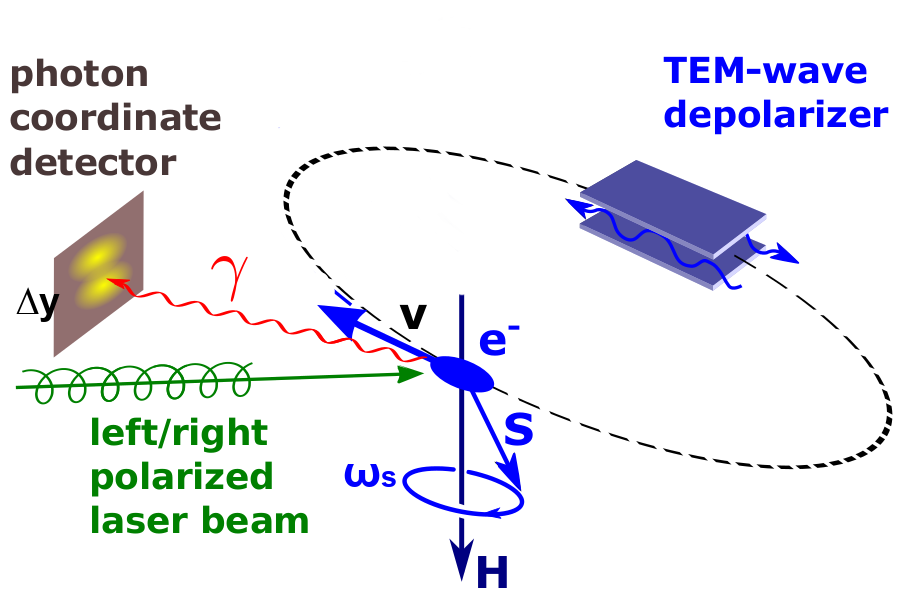
\includegraphics[width = 8cm]{img/mrd-lsrp.png}
		\caption{Принципиальная схема установки по регистрации поляризации электронного пучка. Пучок заряженных частиц (электронов) облучается циркулярно поляризованными фотонами. Происходит обратное комптоновское рассеяние фотонов на электронах, в результате чего образуются высокоэнергитичные (до $1~\GeV$) гамма--кванты, которые регистрируются координатным детектором. Измеряемый эффект есть вертикальное расстояние ($\Delta y$) между центрами пятен, полученных от право и левоциркулярных фотонов .}
		\label{fig:laser_polarimeter_scheme}
	\end{center}
\end{figure}
\vspace{-20pt}
\section{Оценки измеряемого эффекта и точности определения поляризации }
<<Лазерный поляриметр>> коллайдера ВЭПП-4М имеет следующие параметры: 
\begin{itemize}
	\item $\omega_0 = 547 nm$ 
	\item $L = 40 m$
	\item $\Delta V = 2$
\end{itemize}
Подставив их в формулу \ref{eq:pol_effect}, можем получить оценку измеряемого эффекта $\Delta y$, которая составляет около  0.1 мм. Измерение такого малого смещения на первый взгляд представляется затруднительным, однако регистрация большого количества фотонов и определение средней вертикальной координаты по выборке дает намного более точное значение, чем одиночное измерение. Стоит заметить, что координатное разрешение детектора в данном случае может быть и больше величины эффекта, но определение среднего по выборке даст требуемую точность. 